\lab{Iterative Solvers}{Iterative Solvers}
\label{lab:iter_methods}
% Written by Tanner Christensen in collaboration with Dr Emily Evans, Spring 2016

\objective{In this lab, we will talk about the benefits to using iterative solvers
and also implement three popular algorithms: 1) Jacobi Method, 2) Gauss Seidel, 3)
 Successive Over-Relaxation.}

In introductory linear algebra classes, we solve linear systems of the form
$A\mathbf{x} = \mathbf{b}$ by using the inverse, $\mathbf{x} = A^{-1}\mathbf{b}$.
While this is a simple analytic solution, it is not always easily computable.
In linear algebra class, we solve many systems that are no bigger than 4 or 5
dimensions. However in applications, linear systems can sometimes have tens of
thousands of parameters. We will present such a problem in Problem \ref{prob:application}.

With problems of this size, it is no longer feasible to calculate an inverse.
Recall in Lab \ref{lab:complexity} we mentioned that computing the inverse of a
matrix is a $O(n^3)$ calculation. That means it requires somewhere on the order
of 1 trillion floating point operations (FLOPS) to calculate the inverse of a
$10000 \times 10000$ matrix. Additionally, there are situations where too many
floating point errors propogate throughout the caluclations and produce a bad
answer.

Luckily, additional methods have been developed to solve systems of this size.
Though finding an exact solution is either very time intensive or unstable,
iterative methods can give us sufficiently close approximations while taking
much less time.

\section*{Iterative Methods}

The general idea behind any iterative method is make an initial guess, apply some computations or an algorithm to give you a better approximate answer, and repeat
this process until convergence.

In this lab, we will discuss three different methods used to solve large linear
systems of equations. These are the Jacobi Method, the Gauss-Seidel method, and Successive Over-Relaxation.

\section*{Jacobi Method}

To explain the Jacobi Method, we will examine a $ 3 \times 3 $ system.
$$
\begin{matrix}
2x_1 &   &      & - & x_3  & = & 3 \\
-x_1 & + & 3x_2 & + & 2x_3 & = & 3 \\
     & + & x_2  & + & 3x_3 & = & -1 \\
\end{matrix}
$$

\begin{comment}
$$
\begin{matrix}
a_{11}x_1 + a_{12}x_2 + a_{13}x_3 = b_1 \\
a_{21}x_1 + a_{22}x_2 + a_{23}x_3 = b_2 \\
a_{31}x_1 + a_{32}x_2 + a_{33}x_3 = b_3 \\
\end{matrix}
$$
\end{comment}

To complete the first iteration of Jacobi Method, we begin with an initial guess $(x^{(0)}_1, x^{(0)}_2, x^{(0)}_3) = (0,0,0)$. Throughout this lab, we will use
 the notation $x^{(k)}_i$ to denote the $k^{th}$ iteration of the algorithm and
 the $i^{th}$ element of $\mathbf{x}$.

We then compute the next approximation $(x^{(1)}_1, x^{(1)}_2, x^{(1)}_3)$ by
solving for $x^{(1)}_i$ as follows

$$
\begin{matrix}
x^{(1)}_1 & = & \frac{1}{2} ( 3 + x^{(0)}_3)  & = & \frac{1}{2} (3 + 0)     & = & \frac{3}{2} \\
x^{(1)}_2 & = & \frac{1}{3} ( 3 + x^{(0)}_1 - 2x^{(0)}_3) & = & \frac{1}{3} (3 + 0 - 0) & = & 1 \\
x^{(1)}_3 & = & \frac{1}{3} ( -1 - x^{(0)}_2)       & = & \frac{1}{3} (-1 - 0)    & = & -\frac{1}{3} \\
\end{matrix}
$$
So $x^{(1)} = (\frac{3}{2}, 1, -\frac{1}{3})$. This concludes one iteration of
the Jacobi method. Computing $\mathbf{x}^{(2)}$ follows similarly.

$$
\begin{matrix}
x^{(2)}_1 & = & \frac{1}{2} ( 3 + x^{(1)}_3)  & = & \frac{1}{2} (3 - \frac{1}{3})     & = & \frac{4}{3} \\
x^{(2)}_2 & = & \frac{1}{3} ( 3 + x^{(1)}_1 - 2x^{(1)}_3) & = & \frac{1}{3} (3 + \frac{3}{2} + \frac{2}{3}) & = &  \frac{31}{18} \\
x^{(2)}_3 & = & \frac{1}{3} ( -1 - x^{(1)}_2)       & = & \frac{1}{3} (-1 - 1)    & = & -\frac{2}{3} \\
\end{matrix}
$$


\begin{comment}
$$
\begin{matrix}
x^{(1)}_1 = ( b_1 - a_{12}x^{(0)}_2 - a_{13}x^{(0)}_3) / a_{11} \\
x^{(1)}_2 = ( b_1 - a_{21}x^{(0)}_1 - a_{23}x^{(0)}_3) / a_{22} \\
x^{(1)}_3 = ( b_1 - a_{31}x^{(0)}_1 - a_{32}x^{(0)}_2) / a_{33} \\
\end{matrix}
$$
\end{comment}

To find $\mathbf{x}^{(k)}$, we repeat the same process of solving for each
$x^{(k)}_i$ until convergence is reached. For this particular problem,
convergence is reached in 29 iterations.

\begin{center}
\begin{tabular}{ c|c c c  }
          & $x^{(k)}_1$ & $x^{(k)}_2$ & $x^{(k)}_3$ \\
    \hline
    $x^{(0)}$ & 0 & 0 & 0 \\
    %\hline
    $x^{(1)}$ & 1.5 & 1 & -0.33333 \\
    %\hline
    $x^{(2)}$ & 1.33333333 & 1.72222222 & -0.66666667 \\
    $x^{(3)}$ & 1.16666667 & 1.88888889 & -0.90740741 \\
    $x^{(4)}$ & 1.0462963 & 1.99382716 & -0.96296296 \\
    \vdots    & \vdots    & \vdots     & \vdots     \\
    $x^{(28)}$ & 0.99999999 & 2.00000001 & -0.99999999 \\
    $x^{(29)}$ & 1 & 2 & -1 \\
\end{tabular}
\end{center}


\subsection*{Matrix Representation of Jacobi Method}
The iterative steps performed above can be expressed in matrix form. First, we
use the fact that $A = D + L + U$ where,
$$
D = \begin{bmatrix}
a_{11} & 0 & \ldots & 0 \\
0 & a_{22} & \ldots & 0 \\
 \vdots & \vdots & \ddots & \vdots \\
0 & 0 & \ldots & a_{nn} \\
\end{bmatrix}
%
L = \begin{bmatrix}
0 & 0 & \ldots & 0 \\
a_{21} &  0 & \ldots & 0\\
 \vdots & \ddots & \ddots & \vdots \\
a_{n1} & \ldots & a_{n,n-1} & 0 \\
\end{bmatrix}
%
U = \begin{bmatrix}
0 & a_{12} & \ldots & a_{1n} \\
0 & 0 & \ddots & \vdots \\
 \vdots & \vdots & \ddots & a_{n-1,n} \\
0 & 0 & \ldots & 0 \\
\end{bmatrix}.
$$

Now we can make substitutions to get,
$$ A\mathbf{x} = \mathbf{b} $$
$$ (D + L + U)\mathbf{x} = \mathbf{b} $$
$$ D\mathbf{x} = \mathbf{b} - (L+U)\mathbf{x} $$
$$ \mathbf{x} = D^{-1}\mathbf{b} - D^{-1}(L+U)\mathbf{x} $$

With this, we can express our algorithm for iteratively updating $\mathbf{x}$ as,

\begin{equation}
\mathbf{x}^{(k+1)} = D^{-1}b - D^{-1}(L+U)\mathbf{x}^{(k)}
\end{equation}

It is common to see the matrix representation of the Jacobi Method in this form.
However, we can manipulate this equation slightly to make it easier to compute
in Python. Since $A = D + L + U$,

$$\mathbf{x}^{(k+1)} = D^{-1}b - D^{-1}(A-D)\mathbf{x}^{(k)} $$

\begin{equation} \label{eq:jacobi}
\mathbf{x}^{(k+1)} = D^{-1}(b - (A-D)\mathbf{x}^{(k)})
\end{equation}

Since $D$ is a diagonal matrix, $D^{-1}$ is just,

$$
\begin{bmatrix}
\frac{1}{a_{11}} & 0 & \ldots & 0 \\
0 & \frac{1}{a_{22}} & \ldots & 0 \\
 \vdots & \vdots & \ddots & \vdots \\
0 & 0 & \ldots & \frac{1}{a_{nn}} \\
\end{bmatrix}.
$$
Therefore we can avoid computing an inverse. Notice that for this algorithm to
work, the matrix $A$ must have nonzero diagonal entries. We will talk about some
other requirements for convergence in the next section. Additionally, with the
help of array broadcasting we can make a few other adjustments that make it even
more efficient.

\begin{problem} \label{prob:jacobi}
Using Equation \ref{eq:jacobi}, implement the Jacobi Method. Avoid using
\li{la.inv}. Your function should accept a matrix \li{A}, a vector \li{b}, and
an optional parameter \li{tol} with a default value of \li{1e-8}. Additionally,
accept an optional parameter \li{maxiters} to help you catch nonconvergent
systems. Set \li{maxiters} $200$ as default. Your function should return the
solution vector \li{x} as well as an array of all the approximations of \li{x}
at each iteration. If \li{maxiters} is hit, return the current solution. If your
system is non-convergent, you will find that the solutions have increasingly
large entries. Test your function on the example above.

\end{problem}

\subsection*{Convergence of the Jacobi Method}
\begin{definition}
    A matrix $A \in M_n(\mathbb{R})$ is \emph{strictly diagonally dominant} if
    $|a_{ii}| > \sum_{j \neq i} |a_{ij}|$ for all $i = 1,2,\hdots,n$.
\end{definition}

\begin{theorem}
The Jacobi method converges for a matrix $A$ if it is strictly diagonally
dominant.
\end{theorem}

Though this is a small subset of all possible matrices in $M_n(\mathbb{R})$,
these matrices show up often in applications. We will discuss some of these
applications later in this lab.

\begin{problem}
    TODO create plot of b - Ax called %fig:jacobi_convergence
    TODO provide them with a linear system as a .npz file to test it on.
To visualize the converence of the Jacobi method, plot the error at each
approximation. This can be computed by calculating $||Ax_i - b||$ for each
approximation $x_i$. Your plot should be similar to the figure below. TODO
add labels to plot and put the code in plots.py.

\begin{figure}[H]
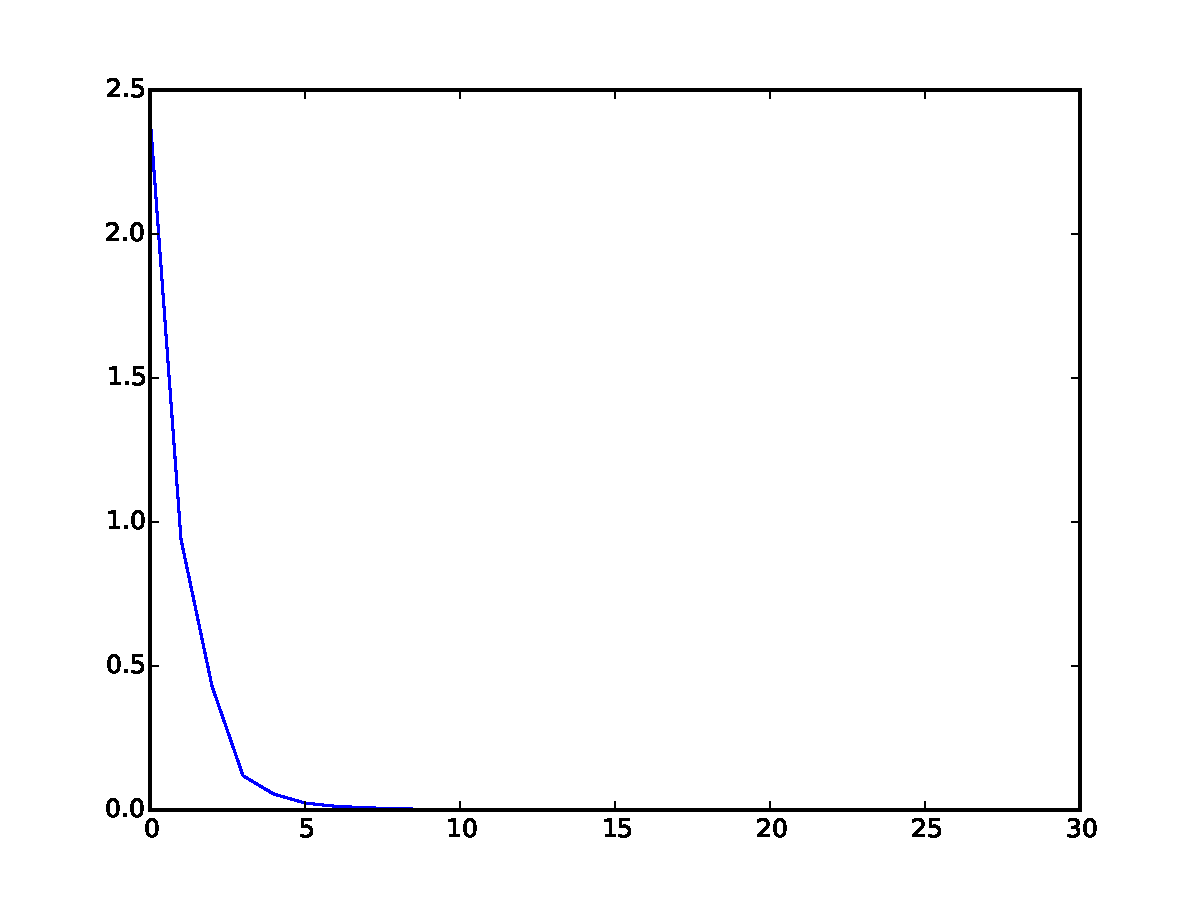
\includegraphics[width=.7\textwidth]{jacobi_convergence.pdf}
\label{fig:jacobi_convergence}
\end{figure}
\end{problem}

\section*{Gauss-Seidel Method}
The Gauss-Seidel Method is quite similar to the Jacobi Method. We will examine
the same system as before. The main difference between Gauss-Seidel and Jacobi
is that in Gauss-Seidel, any new information is used immediately. As with Jacobi,

$$
\begin{matrix}
x^{(1)}_1 & = & \frac{1}{2} ( 3 + x^{(0)}_3)  & = & \frac{1}{2} (3 + 0)     & = & \frac{3}{2} \\
\end{matrix}
$$

But now, we use this updated value of $x^{(1)}_1$ in our calculation of
$x^{(1)}_2$ as follows
$$
\begin{matrix}
x^{(1)}_2 & = & \frac{1}{3} ( 3 + x^{(1)}_1 - 2x^{(0)}_3) & = & \frac{1}{3} (3 + \frac{3}{2} - 0) & = & \frac{3}{2} \\
\end{matrix}
$$

We now can use the updated values of $x^{(1)}_1$ and $x^{(1)}_2$ in our
calculation of $x^{(1)}_3$.
$$
\begin{matrix}
x^{(1)}_3 & = & \frac{1}{3} ( -1 - x^{(1)}_2)       & = & \frac{1}{3} (-1 - \frac{3}{2})    & = & -\frac{5}{6}
\end{matrix}
$$

This process of using what we have calculated right away is called
\emph{forward substitution}. Using forward substitution causes the algorithm to
converge much faster.

\begin{center}
    \begin{tabular} {c | c c c}
        & $x^{(k)}_1$ & $x^{(k)}_2$ & $x^{(k)}_3$ \\
        \hline
          $x^{(0)}$ & 0 & 0 & 0 \\
          %\hline
          $x^{(1)}$ & 1.5 & 1.5 & -0.833333 \\
          %\hline
          $x^{(2)}$ & 1.08333333 & 1.91666667 & -0.97222222 \\
          $x^{(3)}$ & 1.01388889 & 1.98611111 & -0.99537037 \\
          $x^{(4)}$ & 1.00231481 & 1.99768519 & -0.9992284 \\
          \vdots    & \vdots    & \vdots     & \vdots     \\
          $x^{(11)}$ & 1.00000001 & 1.99999999 & -1 \\
          $x^{(12)}$ & 1 & 2 & -1 \\
        \end{tabular}
\end{center}
Notice that Gauss-Seidel converged in less than half as many iterations.

As with the Jacobi Method, we can also represent the Gauss-Seidel method in terms
of matrices. However, we will leave these details for the interested reader to
research further.

As shown above, Gauss-Seidel updates one element of the solution vector at a time.
This process is more generally described by the following equation.

\begin{equation} \label{eq:gauss_seidel_full}
x^{(k+1)}_i = \frac{1}{a_{ii}} \left (b_i - \sum_{j < i}a_{ij}x^{(k+1)}_j - \sum_{j > i}a_{ij}x^{(k)}_j \right )
\end{equation}

Notice that the two sums closely resemble an inner product without the
$i^{\text{th}}$ term. If we update the entries of the vector $\mathbf{x}$ as we
go, this equation can be represented as,

$$
x^{(k+1)}_i = \frac{1}{a_{ii}} \left ( b_i - \left < A_i, \mathbf{x}^{(k)} \right > + a_{ii}x^{(k)}_i \right )
$$
where $A_i$ is the $i^{th}$ row of $A$. This can be simplified further to

\begin{equation} \label{eq:gauss_seidel}
x^{(k+1)}_i = x^{(k)}_i + \frac{1}{a_{ii}} \left ( b_i - \left < A_i, \mathbf{x}^{(k)}\right >\right)
\end{equation}

Making one sweep through all the entries of $x$ completes one iteration. We
continue this same process until convergence is attained.

\begin{problem} \label{prob:gauss_seidel}
Implement the Gauss-Seidel Method using Equation \ref{eq:gauss_seidel}. Your
function should accept a matrix \li{A}, a vector \li{b}, an optional parameter
\li{tol} that defaults to \li{1e-8} and an optional parameter \li{maxiters} that
defaults to $200$. Your function should return the solution vector \li{x} as
well as an array of all the approximations of \li{x} at each iteration.
\end{problem}

\subsection*{Convergence of Gauss-Seidel}
\begin{definition}
    A matrix $A \in M_n(\mathbb(R))$ is \emph{positive definite} if all its
    eigenvalues are positive.
\end{definition}

\begin{theorem}
    The Gauss-Seidel method converges for a matrix $A$ if it is strictly
    diagonally dominant or positive definite.
\end{theorem}

For a treatment on the theory of positive definite matrices, see Chapter ?? of
Volume 1 of the textbook.

\subsection*{Sparse Matrices}
As mentioned in the introduction, there are some systems that have tens of
thousands of parameters. Storing such matrices in memory can become difficult.
For example, when dealing with a system that is $100000 \times 100000$, it
requires around 40 GB to store this matrix in its entirety (4 bytes per entry
$\times$ $10^{10}$ entries).

However, in applications where systems of this size arise, it is also common
that such matrices are sparse. By sparse, we mean that most of the entries in
the matrix are zeros. The \li{scipy.sparse} module provides a solution to this
problem. A \li{sparse} matrix only stores the nonzero values and the positions
of these values. For sufficiently sparse matrices, storing the matrix as a
\li{sparse} matrix may take merely megabytes rather than gigabytes.

There are different kinds of matrices in the \li{sparse} module. Each has their
strengths and weaknesses. In Table \ref{table:sparse_matrices}, we briefly
address the uses of these matrices. We direct the interested reader to the
online documentation for more in-depth information. \url{http://docs.scipy.org/doc/scipy/reference/sparse.html}

\begin{center}
    \begin{tabular} {c | l }
                  & \multicolumn{1}{c}{Intended Uses} \\
        \hline
        \li{coo\_matrix} & Create a matrix using arrays of \\
                         & coordinates and values. Also fast \\
                         & sparse matrix type conversion. \\
        \li{csc\_matrix} & Perform column-based matrix operations. \\
        \li{csr\_matrix} & Perform row-based matrix operations.  \\
        \li{dia\_matrix} & Create a matrix with diagonal structure.  \\
        \li{dok\_matrix} & Access individual elements of the matrix.  \\
        \li{lil\_matrix} & Create a matrix one entry at a time.  \\
        \end{tabular}
\end{center}

The following is a quick example of how the different types of sparse matrices
can be used to optimize performance.

\begin{lstlisting}
# Initialize the matrix using a coo_matrix.
>>> rows = np.array([0,1,2,3,0,2])
>>> cols = np.array([0,1,2,3,1,0])
>>> values = np.array([3,5,4,1,2,1])
>>> A = spar.coo_matrix((values, (rows,cols)), shape=(4,4))

# To visualize the matrix, use .todense(). Keep in mind doing
#   operations on this dense matrix forfeits all sparse-related
#   optimizations.
>>> print A.todense()
matrix([[3, 2, 0, 0],
        [0, 5, 0, 0],
        [1, 0, 4, 0],
        [0, 0, 0, 1]])

# perform matrix multiplicaton after converting to a csr_matrix.
>>> Acsr = A.tocsr()
>>> x = np.array([1,0,-1,2])
>>> b = Acsr.dot(x)
array([3,0,-3,2])

# access individual elements of the matrix after converting to a dok_matrix.
>>> Adok = A.todok()
>>> print Adok[2,0]
1
>>> print Adok[1,1]
5
\end{lstlisting}

Since the \li{coo_matrix} type allows for fast sparse matrix type conversion, it
is usually worth the time and memory to convert to the sparse matrix type that corresponds with the operations you are performing.

Many of the same methods you are used to using with NumPy arrays have similar
functions in the \li{scipy.sparse} module. These methods take advantage of the
sparse structure of the matrices and are, therefore, usually significantly faster.
Note that there is also a \li{scipy.sparse.linalg} module that has linear algebra
methods that have been optimized for sparse matrices. We will use the
\li{scipy.sparse} module more in future labs.

\begin{problem}
To be able to use the Gauss-Seidel method on sparse matrices, you must translate
the code you wrote in \ref{prob:gauss_seidel} from \li{numpy} to \li{scipy.sparse}.
The algorithm is the same, but there are some functions that are named differently between these two packages.

Write a new function that accepts a sparse matrix \li{A}, a NumPy array \li{b}, an optional parameter \li{tol} that defauls to \li{1e-8}, and an optional parameter \li{maxiters} that defaults to 200. Your function should return the solution
vector \li{x} as well as an array of all the approximations of \li{x} at each
iteration. Be sure to use different types of sparse matrices to optimize
performance.
\end{problem}

\section*{Successive Over-Relaxation}
There are some systems that meet the requirements for convergence in the
Gauss-Seidel method that do not converge very quickly. A slightly altered version
of the Gauss-Seidel method has been developed that can result in faster convergence.
This is achieved by introducting a relaxation factor, $\omega$. This method is
called Successive Over-Relaxation. In fact, for many slowly converging iterative processes, convergence can be improved by introducing a relaxation factor.

The iterative equation for Gauss-Seidel, Equation \ref{eq:gauss_seidel_full},
with the introduction of a relaxing factor $\omega$ becomes,

$$
x_i^{(k+1)} = (1 - \omega)x_i^{(k)} + \frac{\omega}{a_{ii}} \left (b_i - \sum_{j < i}a_{ij}x^{(k+1)}_j - \sum_{j > i}a_{ij}x^{(k)}_j \right )
$$

Updating the solution vector $x$ inplace as we did with Gauss-Seidel, this
equation becomes,

\begin{equation} \label{eq:sor}
x^{(k+1)}_i = x^{(k)}_i + \frac{\omega}{a_{ii}} \left ( b_i - \left < A_i, \mathbf{x}^{(k)} \right > \right )
\end{equation}

Equation \ref{eq:sor} follows be simplifying the full analytic equation in the
same way we simplified the Gauss-Seidel method. Notice that when $\omega = 1$,
Successive Over-Relaxation is equivalent to Gauss-Seidel.

\begin{problem}
The choice of $\omega$ can improve the rate of convergence dramatically. However,
it is not always easy to choose the optimal value of $\omega$. To visualize the
effect that different values of $\omega$ has on rate of convergence, do the
following:
\begin{enumerate}
    \item Implement Successive Over-Relaxation. You should be able to write
    this function by changing one line of your code from your Gauss Seidel
    function. Your function should be able to handle sparse matrices.
    \item Plot a graph of the number of iterations required to achieve
    convergence when using various values of $\omega$. Do this for 50
    evenly-spaced values of $\omega$ between 0 and 2. HINT: consider using \li{np.linspace}.
    \item Find what value of $\omega$ is optimal. If this value is not equal to
    1, that means that Successive Over-Relaxation performed better than
    Gauss-Seidel.
\end{enumerate}
\end{problem}

\section*{Application: (whatever the problem is)}
Throughout this lab, we have said there are sparse linear systems that arise in applications that have tens of thousands of parameters. Systems of this size
often arise in Finite Element problems. The theory behind such problems will be
addressed in Volume 4 of the textbook. We now address one such problem.

\begin{problem} \label{prob:application}
TODO Describe the problem they will be solving.

This problem essentially reduces to solving a large linear system.

TODO Figure out how to help them get Dr Evans problem into a sparse matrix on
their computer.

Run the Successive Over-Relaxation method on the problem described above. Set
$\omega = $ (whatever is optimal).

TODO Plot the solution and describe what it means.
\end{problem}
